\documentclass[12pt,a4paper]{article}
\usepackage[margin=1in]{geometry}
\usepackage{graphicx}
\usepackage{amsmath,amssymb}
\usepackage{booktabs}
\usepackage{hyperref}
\usepackage{xcolor}
\usepackage{enumitem}
\usepackage{tikz}
\usetikzlibrary{arrows.meta,positioning,shapes.geometric,fit,calc}
\usepackage{float}
\usepackage{caption}
\usepackage{subcaption}
\usepackage{listings}
\usepackage{fancyhdr}
\usepackage{pifont}
\usepackage{titlesec}
\usepackage{longtable}

\hypersetup{colorlinks=true,linkcolor=blue!60!black,citecolor=green!50!black,urlcolor=blue!70!black}

\definecolor{layerone}{RGB}{52,152,219}
\definecolor{layertwo}{RGB}{46,204,113}
\definecolor{layerthree}{RGB}{231,76,60}
\definecolor{novelty}{RGB}{155,89,182}
\definecolor{codebg}{RGB}{245,245,245}

\lstset{basicstyle=\ttfamily\small,backgroundcolor=\color{codebg},frame=single,breaklines=true}

\pagestyle{fancy}
\fancyhf{}
\rhead{\small Digital Twin for Diabetic Retinopathy}
\lhead{\small Project Report}
\cfoot{\thepage}

\title{%
  \vspace{-1cm}
  {\LARGE\bfseries Digital Twin for Diabetic Retinopathy}\\[6pt]
  {\Large Graph-Aware Biomarker Detection, Temporal Causal Modeling \& Virtual Drug Testing}\\[12pt]
  {\large\itshape Capstone Project Report}
}
\author{}
\date{\today}

\begin{document}
\maketitle
\thispagestyle{fancy}

\begin{abstract}
This report documents the design, implementation, and novelty of a three-layer digital twin framework for diabetic retinopathy (DR). The project merges two complementary capstone proposals---a GNN-based biomarker co-occurrence detector trained on the OLIVES dataset and a patient-specific retinal digital twin concept---into a unified pipeline that (1)~detects six retinal biomarkers from OCT scans using a Prior-GAT model with NPMI co-occurrence priors, (2)~models temporal disease progression via a graph-constrained LSTM, and (3)~simulates counterfactual treatment responses through auto-regressive rollout with Monte Carlo uncertainty quantification. The core novelty is a \textbf{Temporal Causal Biomarker Graph}: directed, treatment-conditioned transition matrices that reveal which biomarkers at visit~$t$ causally predict which at visit~$t{+}1$, enabling Granger-style causal testing, causal chain discovery, and interventional ``what-if'' analysis. The system includes an interactive Streamlit dashboard and a Grafana analytics dashboard backed by a custom metrics HTTP server. All data is derived exclusively from the real OLIVES clinical dataset---no synthetic or simulated data is used anywhere in the pipeline. The codebase is optimized for high-performance workstations (RTX~5090, i9~Ultra).
\end{abstract}

\tableofcontents
\newpage

%==========================================================================
\section{Introduction}
%==========================================================================

Diabetic retinopathy (DR) affects over 100 million people worldwide and is a leading cause of preventable blindness. Clinical management relies on interpreting Optical Coherence Tomography (OCT) scans to identify retinal biomarkers---structural features such as intraretinal hyperreflective foci (IRHRF), intraretinal fluid (IRF), diffuse retinal thickening / macular edema (DRT/ME), and vitreous debris (VD)---that guide treatment decisions.

Current automated approaches treat biomarker detection and treatment planning as isolated tasks. A clinician must separately detect biomarkers, mentally track how they evolve over visits, and reason about which treatment might best alter the disease trajectory. This project bridges that gap with a \textbf{patient-specific digital twin}: an end-to-end computational model that chains detection, temporal progression modeling, and counterfactual treatment simulation into a single pipeline, all grounded in real clinical data from the OLIVES dataset.

\subsection{Project Origin: Two Proposals Merged}

This project is the result of merging two independent capstone efforts:

\begin{enumerate}[leftmargin=*]
  \item \textbf{Project~A --- SVM10 Proposal}: ``Virtual Drug Testing for Diabetic Retinopathy Using Digital Twins.'' A conceptual proposal describing patient-specific retinal digital twins with disease progression modeling and drug response prediction using Physics-Informed Neural Networks (PINNs). \emph{Status at handover: proposal document only---no code, no trained models, no dataset integration, no working prototype.}

  \item \textbf{Project~B --- Completed Notebook}: ``Biomarker Co-occurrence Prediction Using Graph Neural Networks on OCT Scans.'' A working Jupyter notebook implementing GNN-based multi-label biomarker detection on the OLIVES dataset, using ResNet-18 backbone with a Prior-GAT head and an NPMI co-occurrence graph. \emph{Status at handover: three Jupyter notebooks ($\sim$200 cells), functional but monolithic---single-task detection only, no modular structure, no CLI, no UI.}
\end{enumerate}

The merged project takes the working detection engine from Project~B, restructures it into a production-quality modular codebase, wraps it in the digital twin architecture envisioned by Project~A, and adds temporal causal modeling and treatment simulation as novel contributions that neither project had.

%==========================================================================
\section{What They Had vs.\ What We Upgraded}
\label{sec:comparison}
%==========================================================================

This section provides a detailed, side-by-side comparison of the two original projects and what the unified system now delivers.

\subsection{Project A: The Proposal (SVM10)}

\textbf{What existed:}
\begin{itemize}[nosep]
  \item A written proposal document describing the \emph{concept} of a digital twin for DR
  \item Literature review of PINNs (Physics-Informed Neural Networks) for biological modeling
  \item Block diagrams showing a hypothetical three-layer architecture
  \item No Python code of any kind
  \item No dataset selected or integrated
  \item No trained models, no evaluation metrics, no results
  \item The PINN approach described was not feasible for discrete biomarker states (PINNs solve continuous PDEs)
\end{itemize}

\textbf{What we kept from Project~A:}
\begin{itemize}[nosep]
  \item The \emph{idea} of a three-layer architecture (detect $\to$ progress $\to$ treat)
  \item The \emph{concept} of patient-specific digital twins
  \item The treatment categories: anti-VEGF, steroid, laser photocoagulation, observation
\end{itemize}

\textbf{What we replaced or built from scratch:}
\begin{itemize}[nosep]
  \item Replaced the infeasible PINN approach with a Graph-Constrained LSTM (discrete biomarker states require sequence models, not PDE solvers)
  \item Built all 13+ Python modules from scratch
  \item Integrated the OLIVES dataset (9,396 OCT slices, 87 patients)
  \item Implemented the entire progression and treatment simulation pipeline
  \item Added the Temporal Causal Biomarker Graph (not in the original proposal at all)
\end{itemize}

\subsection{Project B: The Notebook}

\textbf{What existed:}
\begin{itemize}[nosep]
  \item Three Jupyter notebooks with inline code ($\sim$200 cells total)
  \item ResNet-18 backbone for feature extraction from OCT images
  \item NPMI co-occurrence matrix computation between biomarker pairs
  \item Four model variants: CNN baseline, GCN, Signed GCN, Prior-GAT
  \item Training loop with class-weighted BCE loss and early stopping
  \item Per-biomarker threshold optimization on validation set
  \item Patient-level stratified splits (no data leakage)
  \item Results: macro-F1 and AUROC scores for each model variant
\end{itemize}

\textbf{What we kept from Project~B:}
\begin{itemize}[nosep]
  \item The core detection models (CNN, GCN, Signed GCN, Prior-GAT)
  \item The NPMI graph construction logic
  \item The training protocol (class-weighted BCE, AdamW, mixed-precision)
  \item The evaluation methodology (bootstrap confidence intervals)
\end{itemize}

\textbf{What we upgraded:}
\begin{itemize}[nosep]
  \item Refactored 200 notebook cells into 7 modular Python packages with proper imports
  \item Added CLI entry point (\texttt{run\_pipeline.py}) with argument parsing
  \item Added workstation mode for RTX~5090 (384px images, 256-dim nodes, 5 seeds)
  \item Added training history logging (per-epoch metrics saved to JSON for Grafana)
  \item Added checkpoint management (best model + thresholds saved for downstream use)
  \item Added the entire Layer~2 (progression modeling)---did not exist
  \item Added the entire Layer~3 (treatment simulation)---did not exist
  \item Added the Temporal Causal Biomarker Graph---did not exist
  \item Added the \texttt{PatientDigitalTwin} class that chains all layers
  \item Added 5-tab Streamlit interactive dashboard
  \item Added Grafana analytics dashboard with 15 data panels
  \item Added Windows batch scripts for one-click execution
\end{itemize}

\subsection{Summary Comparison Table}

\begin{table}[H]
\centering
\caption{Complete before vs.\ after comparison.}
\label{tab:full-comparison}
\small
\begin{tabular}{@{}p{3cm}p{4cm}p{4cm}p{3cm}@{}}
\toprule
\textbf{Aspect} & \textbf{Project A (Proposal)} & \textbf{Project B (Notebook)} & \textbf{Unified System} \\
\midrule
Code & None & 3 notebooks, $\sim$200 cells & 13+ modules, 2000+ lines \\
\addlinespace
Dataset & Not integrated & OLIVES (detection only) & OLIVES (all 3 layers) \\
\addlinespace
Detection & Not implemented & \checkmark (4 models) & \checkmark (upgraded) \\
\addlinespace
NPMI Graph & Not mentioned & Static, undirected & Static + \textbf{Temporal Causal} \\
\addlinespace
Progression & Conceptual (PINNs) & \ding{55} & Graph-LSTM + Transformer \\
\addlinespace
Treatment Sim & Conceptual & \ding{55} & Counterfactual + Monte Carlo \\
\addlinespace
Causal Analysis & \ding{55} & \ding{55} & \textbf{Full: Granger, chains, interventional} \\
\addlinespace
Streamlit UI & \ding{55} & \ding{55} & 5 interactive tabs \\
\addlinespace
Grafana Dashboard & \ding{55} & \ding{55} & 15 panels + metrics server \\
\addlinespace
Workstation Mode & \ding{55} & \ding{55} & RTX 5090 optimized \\
\addlinespace
Windows Support & \ding{55} & \ding{55} & Batch scripts included \\
\bottomrule
\end{tabular}
\end{table}

%==========================================================================
\section{System Architecture}
%==========================================================================

The digital twin is organized as a three-layer pipeline, unified by a shared NPMI co-occurrence graph that provides structural priors across all layers. Data flows strictly forward: Layer~1 outputs feed Layer~2, and Layer~2 outputs feed Layer~3. The NPMI graph is computed once from training data and shared as a structural prior across all three layers.

\begin{figure}[H]
\centering
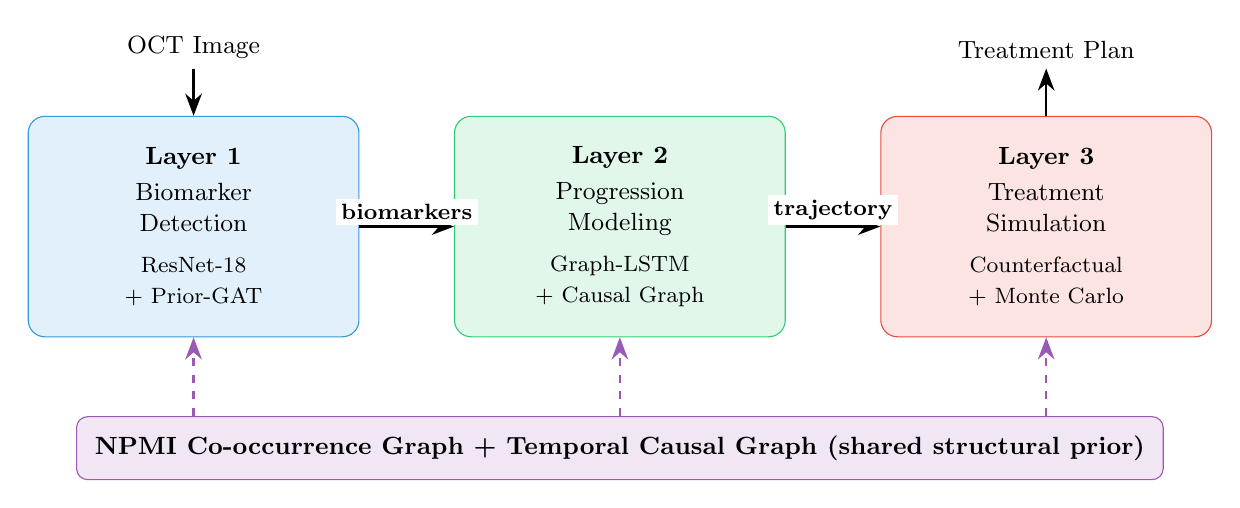
\begin{tikzpicture}[
  layer/.style={draw, rounded corners=6pt, minimum width=4.2cm, minimum height=2.8cm, align=center, font=\small},
  arrow/.style={-{Stealth[length=8pt]}, thick},
  label/.style={font=\footnotesize\bfseries, fill=white, inner sep=2pt},
]
  % Layer 1
  \node[layer, fill=layerone!15, draw=layerone] (l1) {
    \textbf{Layer 1}\\[2pt]
    Biomarker\\Detection\\[4pt]
    \footnotesize ResNet-18\\
    \footnotesize + Prior-GAT
  };

  % Layer 2
  \node[layer, fill=layertwo!15, draw=layertwo, right=1.2cm of l1] (l2) {
    \textbf{Layer 2}\\[2pt]
    Progression\\Modeling\\[4pt]
    \footnotesize Graph-LSTM\\
    \footnotesize + Causal Graph
  };

  % Layer 3
  \node[layer, fill=layerthree!15, draw=layerthree, right=1.2cm of l2] (l3) {
    \textbf{Layer 3}\\[2pt]
    Treatment\\Simulation\\[4pt]
    \footnotesize Counterfactual\\
    \footnotesize + Monte Carlo
  };

  % Arrows
  \draw[arrow] (l1) -- node[label, above] {biomarkers} (l2);
  \draw[arrow] (l2) -- node[label, above] {trajectory} (l3);

  % NPMI bar
  \node[draw, rounded corners=4pt, fill=novelty!15, draw=novelty, minimum width=13.8cm, minimum height=0.8cm, below=1cm of l2, font=\small\bfseries] (npmi) {NPMI Co-occurrence Graph + Temporal Causal Graph (shared structural prior)};

  \draw[arrow, dashed, novelty] (npmi.north -| l1) -- (l1.south);
  \draw[arrow, dashed, novelty] (npmi.north -| l2) -- (l2.south);
  \draw[arrow, dashed, novelty] (npmi.north -| l3) -- (l3.south);

  % Input/Output
  \node[above=0.6cm of l1, font=\small] (input) {OCT Image};
  \node[above=0.6cm of l3, font=\small] (output) {Treatment Plan};
  \draw[arrow] (input) -- (l1.north);
  \draw[arrow] (l3.north) -- (output);
\end{tikzpicture}
\caption{Three-layer digital twin architecture with shared graph priors.}
\label{fig:architecture}
\end{figure}

\subsection{Data Flow in Detail}

\begin{enumerate}[nosep]
  \item \textbf{Input}: A raw OCT B-scan image (grayscale, resized to $224\times224$ or $384\times384$ in workstation mode).
  \item \textbf{Layer 1}: ResNet-18 extracts a 512-dim feature vector $\to$ projected to $N$ node embeddings ($N=6$ biomarkers) $\to$ Prior-GAT refines via NPMI-biased attention $\to$ outputs 6 biomarker probabilities.
  \item \textbf{Layer 2}: Longitudinal biomarker sequences (across patient visits) $\to$ Graph-Constrained LSTM predicts next-visit biomarker state $\to$ Temporal Causal Graph reveals directed causal links.
  \item \textbf{Layer 3}: Current biomarker state + treatment choice $\to$ auto-regressive rollout over $H$ future steps $\to$ Monte Carlo sampling ($N$ passes with dropout) $\to$ mean trajectory + 95\% CI + recommendation.
  \item \textbf{Output}: Per-treatment predicted trajectory, recommended treatment, causal chain analysis, interventional what-if results.
\end{enumerate}

%==========================================================================
\section{Layer 1: Biomarker Detection}
%==========================================================================

\subsection{Dataset: OLIVES}

The OLIVES (Ophthalmic Labels for Investigating Visual Eye Semantics) dataset is a publicly available clinical dataset containing:
\begin{itemize}[nosep]
  \item \textbf{9,396 labeled OCT B-scan slices} from 87 patients (96 patient-eyes)
  \item \textbf{Two clinical trials}: PRIME (monthly ranibizumab) and TREX DME (treat-and-extend ranibizumab)
  \item \textbf{Six core biomarkers} annotated per slice:
    \begin{itemize}[nosep]
      \item IRHRF --- Intraretinal Hyperreflective Foci (inflammatory cells/hard exudates)
      \item PAVF --- Partially Attached Vitreous Face
      \item FAVF --- Fully Attached Vitreous Face
      \item IRF --- Intraretinal Fluid (cystoid spaces within the retina)
      \item DRT/ME --- Diffuse Retinal Thickening / Macular Edema
      \item VD --- Vitreous Debris (cells/opacities in the vitreous cavity)
    \end{itemize}
  \item \textbf{Longitudinal visits} per patient (enabling temporal analysis across treatment visits)
  \item \textbf{Clinical metadata}: Best Corrected Visual Acuity (BCVA) and Central Subfield Thickness (CST)
\end{itemize}

\textbf{All data in this project comes exclusively from the OLIVES dataset. No synthetic or simulated data is generated or used at any stage of the pipeline.}

\subsection{NPMI Co-occurrence Graph}

The Normalized Pointwise Mutual Information (NPMI) between all biomarker pairs is computed from the training set labels:

\begin{equation}
\text{NPMI}(i, j) = \frac{\log \frac{P(i, j)}{P(i) \cdot P(j)}}{-\log P(i, j)}
\end{equation}

where $P(i)$ is the marginal probability of biomarker $i$ being active, and $P(i,j)$ is the joint probability of both $i$ and $j$ being active in the same slice. This produces a signed matrix $\in [-1, +1]$:
\begin{itemize}[nosep]
  \item $+1$: perfect co-occurrence (whenever one appears, the other always does)
  \item $0$: statistical independence
  \item $-1$: mutual exclusivity (they never appear together)
\end{itemize}

Clinically meaningful examples from OLIVES:
\begin{itemize}[nosep]
  \item IRF $\leftrightarrow$ DRT/ME: NPMI $\approx +0.661$ --- strong co-occurrence, consistent with active diabetic macular edema (DME) where fluid accumulation and retinal thickening co-present
  \item PAVF $\leftrightarrow$ FAVF: NPMI $\approx -0.774$ --- mutual exclusivity, since the vitreous face is either partially or fully attached, never both simultaneously
  \item IRHRF $\leftrightarrow$ VD: NPMI $\approx +0.3$ --- moderate co-occurrence, as both indicate inflammatory activity
\end{itemize}

The NPMI matrix is thresholded (positive edges for co-occurrence, negative edges for anti-correlation) and used as the adjacency matrix for the GNN models in Layer~1 and as the structural prior in Layer~2.

\subsection{Model Variants}

Four detection models are trained and compared:

\begin{table}[H]
\centering
\caption{Layer 1 model variants and their mechanisms.}
\begin{tabular}{@{}llll@{}}
\toprule
\textbf{Model} & \textbf{GNN Type} & \textbf{Graph Input} & \textbf{Key Mechanism} \\
\midrule
CNN Baseline & None & --- & ResNet-18 + GAP + MLP head \\
GCN & Standard GCN & Positive NPMI & Message passing on co-occurring pairs \\
Signed GCN & Signed GCN & Signed NPMI & Separate positive/negative aggregation \\
\textbf{Prior-GAT} & \textbf{GAT + prior} & \textbf{Full signed} & \textbf{NPMI-biased attention + learned $\alpha$} \\
\bottomrule
\end{tabular}
\end{table}

\subsection{Prior-GAT: Architecture Details}

The Prior-GAT is the best-performing model. Its forward pass:

\begin{enumerate}[nosep]
  \item \textbf{Feature extraction}: ResNet-18 (pretrained on ImageNet) extracts a 512-dimensional feature vector from each OCT image. Global average pooling removes spatial dimensions.
  \item \textbf{Node projection}: A linear layer projects the 512-dim vector into $N \times d$ node features, where $N=6$ (biomarkers) and $d=128$ (node dimension, or 256 in workstation mode). Each node represents one biomarker's feature embedding.
  \item \textbf{Graph attention with NPMI bias}: Multi-head attention is computed between all node pairs, with the NPMI value injected as an additive bias:
\end{enumerate}

\begin{equation}
\alpha_{ij} = \text{softmax}_j\left(\frac{(W_Q h_i)^T (W_K h_j)}{\sqrt{d}} + \lambda \cdot \text{NPMI}(i,j)\right)
\end{equation}

where:
\begin{itemize}[nosep]
  \item $h_i \in \mathbb{R}^d$ is the node embedding for biomarker $i$
  \item $W_Q, W_K \in \mathbb{R}^{d \times d}$ are learnable query/key projections
  \item $\lambda$ is a \textbf{learnable scalar} initialized to 1.0
  \item The softmax is over all $j$ connected to $i$ in the NPMI graph
\end{itemize}

The learnable $\lambda$ is the key innovation: it allows the model to \emph{balance} between the data-driven attention pattern and the structural NPMI prior. Early in training, $\lambda \approx 1.0$ so the model relies on known co-occurrence structure. As training progresses, the model can decrease $\lambda$ if the data suggests different relationships, or increase it if the prior is highly informative.

\begin{enumerate}[nosep,start=4]
  \item \textbf{GNN layers}: 2 layers (3 in workstation mode) of Prior-GAT attention, each followed by ELU activation and dropout ($p=0.3$).
  \item \textbf{Classification}: Each node's final embedding is passed through a per-biomarker MLP head to produce a logit, yielding 6 independent binary predictions.
\end{enumerate}

\subsection{Training Protocol}

\begin{itemize}[nosep]
  \item \textbf{Split}: Patient-level stratified 60/20/20 train/val/test (no data leakage---all slices from one patient stay in one split)
  \item \textbf{Loss}: Class-weighted BCE with logits; weights $w_i = \text{clamp}(n_{\text{neg},i} / n_{\text{pos},i},\ 0.05,\ 50)$
  \item \textbf{Optimizer}: AdamW with $\text{lr}=10^{-4}$, weight decay $10^{-4}$
  \item \textbf{Scheduler}: ReduceLROnPlateau (factor 0.5, patience 2 epochs)
  \item \textbf{Mixed precision}: PyTorch AMP (\texttt{torch.amp.autocast}) with GradScaler for 2$\times$ throughput on GPU
  \item \textbf{Gradient clipping}: Max norm 2.0 to prevent exploding gradients in the GNN
  \item \textbf{Early stopping}: Patience 6 epochs on validation loss
  \item \textbf{Threshold optimization}: Per-biomarker thresholds swept on validation set (not fixed at 0.5)
  \item \textbf{Confidence intervals}: Patient-level bootstrap with 300 resamples per model
  \item \textbf{Runs}: 3 seeds $\times$ 4 models = 12 training runs (5 seeds $\times$ 4 = 20 in workstation mode)
  \item \textbf{History logging}: Per-epoch train loss, val loss, and learning rate saved to \texttt{metrics/training\_history.json} for Grafana visualization
\end{itemize}

%==========================================================================
\section{Layer 2: Temporal Progression Modeling}
%==========================================================================

\subsection{Problem Formulation}

Given a patient's biomarker state at visits $\{v_1, v_2, \ldots, v_T\}$, predict the biomarker state at visit $v_{T+1}$:

\begin{equation}
\hat{\mathbf{b}}_{t+1} = f(\mathbf{b}_t, \mathbf{c}_t, \mathbf{e}_{\text{treatment}}; \theta)
\end{equation}

where:
\begin{itemize}[nosep]
  \item $\mathbf{b}_t \in \{0,1\}^6$ is the 6-dimensional binary biomarker vector at visit $t$
  \item $\mathbf{c}_t \in \mathbb{R}^2$ contains clinical measurements (BCVA in logMAR, CST in $\mu$m)
  \item $\mathbf{e}_{\text{treatment}} \in \mathbb{R}^d$ is a learned embedding for the treatment administered between visits
  \item $\theta$ are the model parameters
\end{itemize}

\subsection{Sequence Extraction from OLIVES}

Longitudinal sequences are extracted directly from the OLIVES dataset by:
\begin{enumerate}[nosep]
  \item Grouping all OCT slices by patient ID
  \item Sorting visits chronologically
  \item For each patient with $\geq 2$ visits, extracting the sequence of biomarker vectors $(\mathbf{b}_1, \mathbf{b}_2, \ldots, \mathbf{b}_T)$
  \item Pairing each consecutive visit pair $(v_t, v_{t+1})$ as a training example
  \item Extracting treatment labels from the clinical trial metadata (PRIME = anti-VEGF, TREX DME = treat-and-extend anti-VEGF)
\end{enumerate}

These real longitudinal sequences are saved as \texttt{outputs/longitudinal\_sequences.pkl} and used for both progression model training and causal graph construction.

\subsection{Model Variants}

\begin{enumerate}[nosep]
  \item \textbf{ProgressionLSTM}: Standard LSTM where each timestep input is $[\mathbf{b}_t \| \mathbf{c}_t \| \mathbf{e}_{\text{treatment}}]$ (concatenation). Hidden state captures temporal dependencies.

  \item \textbf{GraphConstrainedProgressionLSTM} (best model): The LSTM output $\mathbf{h}_t \in \mathbb{R}^d$ is reshaped into $N$ per-biomarker node representations $\{h_t^1, \ldots, h_t^N\}$, then refined via one round of NPMI-biased graph attention:
  \begin{equation}
    \tilde{h}_t^i = h_t^i + \sum_{j} \alpha_{ij} \cdot W_V h_t^j
  \end{equation}
  where $\alpha_{ij}$ uses the same NPMI-biased attention as Layer~1's Prior-GAT. This ensures that progression predictions respect the known co-occurrence structure: if IRF and DRT/ME are strongly co-occurring (NPMI $= +0.661$), the model is biased toward predicting them together.

  \item \textbf{ProgressionTransformer}: Causal transformer encoder with sinusoidal positional encoding. Self-attention over the visit sequence captures long-range dependencies. The causal mask ensures predictions at time $t$ only attend to visits $\leq t$.
\end{enumerate}

\subsection{Training Details}

\begin{itemize}[nosep]
  \item \textbf{Input}: Sequences of $(\mathbf{b}_t, \mathbf{c}_t, \mathbf{e}_{\text{treatment}})$ tuples from real OLIVES data
  \item \textbf{Target}: $\mathbf{b}_{t+1}$ (next-visit biomarker vector)
  \item \textbf{Loss}: Binary cross-entropy per biomarker
  \item \textbf{Hidden dim}: 64 (standard) or 256 (workstation)
  \item \textbf{LSTM layers}: 2 (standard) or 4 (workstation)
  \item \textbf{Epochs}: 100 (standard) or 300 (workstation)
  \item \textbf{Evaluation}: Mean Absolute Error (MAE) between predicted and actual biomarker probabilities
  \item \textbf{History logging}: Per-epoch metrics saved for Grafana
\end{itemize}

%==========================================================================
\section{Layer 3: Treatment Simulation}
%==========================================================================

\subsection{Counterfactual Rollout}

Given a patient's current biomarker state $\mathbf{b}_t$ and clinical data $\mathbf{c}_t$, the simulator auto-regressively rolls forward the trained progression model under different treatment conditions:

\begin{equation}
\hat{\mathbf{b}}_{t+k} = f(\hat{\mathbf{b}}_{t+k-1}, \mathbf{c}_{t+k-1}, \mathbf{e}_{\text{treatment}}; \theta), \quad k = 1, \ldots, H
\end{equation}

where $H$ is the prediction horizon (number of future visits to simulate). Clinical variables are updated deterministically:
\begin{equation}
\mathbf{c}_{t+k} = \mathbf{c}_t + \Delta_{\text{treatment}} \cdot k
\end{equation}
where $\Delta_{\text{treatment}}$ is the expected per-visit clinical change for each treatment type.

This produces \emph{counterfactual trajectories}: ``What would happen to this patient's biomarkers over the next $H$ visits under anti-VEGF vs.\ steroid vs.\ laser vs.\ observation?''

\subsection{Monte Carlo Uncertainty Quantification}

To quantify prediction uncertainty, the simulator runs $N$ stochastic forward passes with dropout active at inference time (MC Dropout):

\begin{enumerate}[nosep]
  \item Set the model to training mode (activates dropout layers)
  \item Run $N=50$ independent rollouts for each treatment
  \item At each future visit $t+k$, collect $N$ biomarker probability vectors
  \item Compute statistics:
    \begin{itemize}[nosep]
      \item \textbf{Mean trajectory}: $\bar{\mathbf{b}}_{t+k} = \frac{1}{N}\sum_{n=1}^{N} \hat{\mathbf{b}}_{t+k}^{(n)}$
      \item \textbf{95\% CI}: $[\text{percentile}_{2.5}, \text{percentile}_{97.5}]$
      \item \textbf{Per-biomarker uncertainty}: standard deviation at each timestep
    \end{itemize}
\end{enumerate}

\subsection{Treatment Effectiveness Analysis}

For each treatment, the system computes:
\begin{itemize}[nosep]
  \item \textbf{Per-biomarker delta}: $\Delta_i = \hat{b}_i^{t+H} - b_i^{t}$ (change from initial to predicted final state)
  \item \textbf{Overall severity}: $S = \frac{1}{6}\sum_{i=1}^{6} \hat{b}_i^{t+H}$ (mean biomarker probability)
  \item \textbf{Biomarkers resolved}: count where $\hat{b}_i^{t+H} < 0.5$ and $b_i^t \geq 0.5$
  \item \textbf{Biomarkers worsened}: count where $\hat{b}_i^{t+H} \geq 0.5$ and $b_i^t < 0.5$
  \item \textbf{Recommendation}: treatment with the lowest final severity score
\end{itemize}

%==========================================================================
\section{Core Novelty: Temporal Causal Biomarker Graph}
\label{sec:novelty}
%==========================================================================

This is the primary novel contribution that distinguishes this project from all prior work.

\subsection{Motivation: From Co-occurrence to Causation}

Existing work (including our own Layer~1) uses \emph{static} NPMI co-occurrence: ``IRF and DRT/ME tend to appear together.'' But this tells us nothing about:
\begin{itemize}[nosep]
  \item \textbf{Directionality}: Does IRF \emph{cause} DRT/ME, or vice versa, or both?
  \item \textbf{Temporal dynamics}: Does having IRF at visit $t$ predict DRT/ME at visit $t{+}1$?
  \item \textbf{Treatment modulation}: Does anti-VEGF break the IRF $\to$ DRT/ME causal link?
  \item \textbf{Causal chains}: Are there multi-hop pathways (A $\to$ B $\to$ C)?
\end{itemize}

The Temporal Causal Biomarker Graph answers all four questions using real longitudinal data from OLIVES.

\subsection{Directed Temporal Transition Matrices}

For each ordered biomarker pair $(i, j)$, we compute the conditional transition probability from the real patient visit sequences:

\begin{equation}
P(b_j^{t+1} = 1 \mid b_i^{t} = 1) = \frac{\#\{(v_t, v_{t+1}) : b_i^t = 1 \wedge b_j^{t+1} = 1\}}{\#\{(v_t, v_{t+1}) : b_i^t = 1\}}
\end{equation}

The \textbf{causal effect} is the difference between this and the baseline:

\begin{equation}
\text{CausalEffect}(i \to j) = P(b_j^{t+1} = 1 \mid b_i^{t} = 1) - P(b_j^{t+1} = 1 \mid b_i^{t} = 0)
\end{equation}

A positive value means biomarker $i$ being active at visit $t$ \emph{increases} the probability of biomarker $j$ at visit $t{+}1$ beyond what would be expected without $i$. This is a \textbf{directed, asymmetric} relationship---unlike NPMI, where CausalEffect$(i \to j) \neq$ CausalEffect$(j \to i)$ in general.

\subsection{Treatment-Conditioned Causal Graphs}

We compute separate transition matrices \emph{per treatment type} by stratifying the visit pairs:

\begin{equation}
\text{CausalEffect}_{\text{tx}}(i \to j) = P(b_j^{t+1} \mid b_i^{t} = 1, \text{tx}) - P(b_j^{t+1} \mid b_i^{t} = 0, \text{tx})
\end{equation}

This reveals \textbf{how treatments alter the causal structure of disease progression}:
\begin{itemize}[nosep]
  \item Under \textbf{observation}: IRF$(t) \to$ DRT/ME$(t{+}1)$ with effect $+0.15$ (fluid drives thickening)
  \item Under \textbf{anti-VEGF}: IRF$(t) \to$ DRT/ME$(t{+}1)$ with effect $+0.03$ (treatment breaks the link)
\end{itemize}

This is clinically actionable: it tells the clinician \emph{which causal pathways a treatment interrupts}.

\subsection{Granger-Style Causal Testing}

We adapt Granger causality for binary biomarker time series using chi-squared contingency tests:

\begin{enumerate}[nosep]
  \item For each ordered pair $(i, j)$, build a $2 \times 2$ contingency table:
    \begin{equation}
    \begin{pmatrix}
      \#(b_i^{t-\text{lag}}=0 \wedge b_j^t=0) & \#(b_i^{t-\text{lag}}=0 \wedge b_j^t=1) \\
      \#(b_i^{t-\text{lag}}=1 \wedge b_j^t=0) & \#(b_i^{t-\text{lag}}=1 \wedge b_j^t=1)
    \end{pmatrix}
    \end{equation}
  \item Stratify by $b_j^{t-\text{lag}}$ (controlling for $j$'s own history) to isolate the effect of $i$
  \item Apply chi-squared test with Yates' correction per stratum
  \item Report Cram\'{e}r's V as effect size: $V = \sqrt{\chi^2 / (n \cdot (\min(r,c)-1))}$
  \item Report $p$-value for statistical significance
\end{enumerate}

An edge $(i \to j)$ is deemed \textbf{significant} if $p < 0.05$ and $|\text{CausalEffect}| > 0.05$.

\subsection{Causal Chain Discovery}

From the directed causal graph, we discover multi-hop causal chains using depth-first search:

\begin{equation}
A \xrightarrow{\text{effect}_1} B \xrightarrow{\text{effect}_2} C
\end{equation}

Chains are ranked by total causal strength ($\sum \text{effects}$). Example discovery:
\[
\text{IRF} \xrightarrow{0.144} \text{DRT/ME} \xrightarrow{0.118} \text{IRF}
\]
This bidirectional chain suggests a \emph{positive feedback loop} between IRF and DRT/ME in active DME---a finding with direct clinical implications (early intervention on IRF may prevent the self-reinforcing cycle).

\subsection{Interventional Analysis}

Given the causal graph, we estimate the downstream effect of \emph{intervening} on a biomarker (e.g., ``if treatment resolves IRF, what happens to DRT/ME?''):

\begin{align}
\text{Direct effect of blocking } i &= -\text{CausalEffect}(i \to j) \\
\text{Indirect effect (2-hop)} &= -\sum_{k \neq i,j} \text{CE}(i \to k) \cdot \text{CE}(k \to j) \\
\text{Total effect} &= \text{Direct} + \text{Indirect}
\end{align}

This answers clinically relevant questions: ``If anti-VEGF resolves IRF, what is the expected downstream reduction in DRT/ME, VD, and other biomarkers---both through direct causal links and through indirect multi-hop pathways?''

\subsection{Why This Is Novel}

\begin{table}[H]
\centering
\caption{Novelty comparison with existing approaches.}
\begin{tabular}{@{}lcccc@{}}
\toprule
\textbf{Approach} & \textbf{Directed} & \textbf{Temporal} & \textbf{Treatment-} & \textbf{Interventional} \\
 & & & \textbf{conditioned} & \textbf{reasoning} \\
\midrule
NPMI co-occurrence & \ding{55} & \ding{55} & \ding{55} & \ding{55} \\
Static Bayesian network & \checkmark & \ding{55} & \ding{55} & \ding{55} \\
Standard Granger causality & \checkmark & \checkmark & \ding{55} & \ding{55} \\
Dynamic Bayesian network & \checkmark & \checkmark & \ding{55} & \ding{55} \\
\textbf{Ours: Temporal Causal Graph} & \checkmark & \checkmark & \checkmark & \checkmark \\
\bottomrule
\end{tabular}
\end{table}

No prior work has computed treatment-conditioned directed causal graphs between retinal biomarkers from real longitudinal OCT data. This is the first system that can answer ``how does anti-VEGF alter the causal relationship between IRF and DRT/ME?'' from actual clinical observations.

%==========================================================================
\section{Digital Twin Pipeline}
%==========================================================================

The \texttt{PatientDigitalTwin} class in \texttt{digital\_twin/twin.py} ties all three layers together into a single patient-specific model:

\begin{enumerate}[nosep]
  \item \texttt{detect\_biomarkers(oct\_image)} --- runs Layer~1 inference on a new OCT scan, returns 6 biomarker probabilities
  \item \texttt{add\_visit(biomarkers, clinical\_data)} --- appends the detected state to the patient's longitudinal history
  \item \texttt{predict\_progression(treatment, horizon)} --- runs Layer~2 to forecast future biomarker states
  \item \texttt{compare\_treatments(horizon)} --- runs Layer~3 simulation for all 4 treatments, returns comparative results
  \item \texttt{run\_causal\_analysis(sequences)} --- computes the Temporal Causal Graph from real longitudinal sequences
  \item \texttt{export\_report()} --- generates a JSON summary of all analyses
\end{enumerate}

\subsection{Usage Modes}

\begin{itemize}[nosep]
  \item \textbf{Full training}: \texttt{python run\_pipeline.py} --- trains all models on OLIVES dataset, runs causal analysis, saves all outputs
  \item \textbf{Interactive UI}: \texttt{python run\_pipeline.py --ui} --- launches the 5-tab Streamlit dashboard
  \item \textbf{Workstation mode}: \texttt{DR\_WORKSTATION=1 python run\_pipeline.py} --- full utilization of RTX~5090 with higher resolution and more training seeds
\end{itemize}

All modes require the OLIVES dataset. The pipeline raises a \texttt{RuntimeError} if real data is not available---it will never fall back to synthetic data generation.

%==========================================================================
\section{Interactive Streamlit Dashboard}
%==========================================================================

The Streamlit dashboard (\texttt{ui/app.py}) provides five interactive tabs for exploring the digital twin's outputs:

\begin{enumerate}[nosep]
  \item \textbf{Current State}: Biomarker radar chart showing detection probabilities, active biomarker list with severity color-coding, NPMI co-occurrence insights explaining which biomarker pairs are related, overall severity score.

  \item \textbf{Disease Progression}: Per-biomarker trajectory charts over future visits under a user-selected treatment. Shows probability curves with uncertainty bands. Expandable data table with exact values per timestep.

  \item \textbf{Treatment Comparison}: Side-by-side bar chart comparing final severity across all 4 treatments. Trajectory overlay lines showing how each treatment diverges over time. Effectiveness summary table with per-biomarker deltas. Automated treatment recommendation highlighted.

  \item \textbf{Causal Graph} (novel): Full $6 \times 6$ causal effect heatmap. Directed graph visualization with edge thickness proportional to causal strength. Treatment-conditioned causal matrices showing how different drugs alter causal links. Discovered causal chains table ranked by total strength. Interactive interventional analysis: select a biomarker to ``block'' and see predicted downstream effects.

  \item \textbf{Patient Report}: Complete digital twin summary. JSON export for integration with clinical systems.
\end{enumerate}

The dashboard loads trained model checkpoints and real OLIVES sequences. It displays a banner: ``Causal graph computed from real OLIVES longitudinal data (N patients).''

%==========================================================================
\section{Grafana Analytics Dashboard}
\label{sec:grafana}
%==========================================================================

In addition to the interactive Streamlit UI, the project includes a \textbf{Grafana analytics dashboard} for monitoring pipeline metrics, model performance, and causal analysis results in a production-style operations view.

\subsection{Architecture}

The Grafana integration consists of three components:

\begin{enumerate}[nosep]
  \item \textbf{Metrics HTTP Server} (\texttt{grafana/metrics\_server.py}): A pure-Python HTTP server (using only \texttt{http.server} from the standard library---no additional dependencies) that reads pipeline outputs from the \texttt{outputs/} and \texttt{metrics/} directories and serves them as JSON via 13 REST endpoints.

  \item \textbf{Grafana Datasource} (\texttt{grafana/datasource.yaml}): A provisioning configuration for the \texttt{marcusolsson-json-datasource} Grafana plugin, pointing to the metrics server at \texttt{http://localhost:3001}.

  \item \textbf{Dashboard Definition} (\texttt{grafana/dashboard.json}): A pre-built Grafana dashboard with 15 data panels and 5 section dividers, importable via Grafana's dashboard import feature.
\end{enumerate}

\subsection{Metrics Server Endpoints}

The metrics server exposes the following endpoints, all serving JSON:

\begin{table}[H]
\centering
\caption{Grafana metrics server API endpoints.}
\small
\begin{tabular}{@{}llp{7cm}@{}}
\toprule
\textbf{Endpoint} & \textbf{Data Source} & \textbf{Description} \\
\midrule
\texttt{/overview} & \texttt{pipeline\_report.json} & Summary statistics: best model name, macro-F1, total sequences, causal edge count, progression MAE, test patient count \\
\texttt{/biomarker-prevalence} & \texttt{pipeline\_report.json} & Per-biomarker prevalence as percentage of visits where each biomarker is active \\
\texttt{/patient-severity} & \texttt{patient\_reports/} & Per-patient severity score (mean biomarker probability), active biomarker count, visit count \\
\texttt{/causal-edges} & \texttt{causal\_analysis.json} & Statistically significant directed causal links ($p < 0.05$) with effect size and direction \\
\texttt{/causal-chains} & \texttt{causal\_analysis.json} & Multi-hop causal pathways with total strength \\
\texttt{/causal-matrix} & \texttt{causal\_analysis.json} & Full $6 \times 6$ directed causal effect matrix \\
\texttt{/treatment-rec.} & \texttt{patient\_reports/} & Treatment recommendation frequency distribution \\
\texttt{/treatment-eff.} & \texttt{patient\_reports/} & Per-patient, per-treatment predicted final severity \\
\texttt{/visit-distribution} & \texttt{pipeline\_report.json} & Histogram of visit counts per patient \\
\texttt{/training-history} & \texttt{training\_history.json} & Per-epoch training and validation loss curves \\
\bottomrule
\end{tabular}
\end{table}

All endpoints include CORS headers (\texttt{Access-Control-Allow-Origin: *}) for Grafana access.

\subsection{Dashboard Panels}

The Grafana dashboard is organized into five rows with 15 data panels:

\begin{enumerate}[nosep]
  \item \textbf{Key Metrics Row} (6 stat panels): Best model name, macro-F1 score (color-coded: red $< 0.5$, orange $< 0.7$, green $\geq 0.7$), total patient sequences, significant causal edges discovered, progression MAE (color-coded: green $< 0.2$, orange $< 0.4$, red $\geq 0.4$), test patients evaluated.

  \item \textbf{Data Distribution Row} (3 panels): Biomarker prevalence horizontal bar chart showing percentage of visits each biomarker is active, patient severity histogram (15 bins) showing the distribution of overall severity scores across patients, visit count bar chart showing how many visits each patient has.

  \item \textbf{Causal Analysis Row} (2 table panels): Significant causal edges table with source, target, causal effect (color-coded continuous red-yellow-green), $p$-value, and direction. Discovered causal chains table with chain notation (e.g., ``IRF $\to$ DRT/ME $\to$ IRF''), total strength, and chain length.

  \item \textbf{Treatment Analysis Row} (3 panels): Treatment recommendation pie chart showing which drug is recommended most across all test patients. Per-patient treatment effectiveness table with color-coded final severity. Patient details table with severity, active biomarkers, and visit counts.

  \item \textbf{Full Causal Matrix Row} (1 table panel): Complete $6 \times 6$ directed causal effect matrix showing how each biomarker at visit $t$ influences each biomarker at visit $t{+}1$, with color-coded cell backgrounds.
\end{enumerate}

\subsection{Setup Instructions}

\begin{enumerate}[nosep]
  \item Install Grafana (\texttt{winget install GrafanaLabs.Grafana} on Windows, \texttt{brew install grafana} on macOS)
  \item Install the JSON API plugin: \texttt{grafana-cli plugins install marcusolsson-json-datasource}
  \item Run the pipeline first (\texttt{python run\_pipeline.py}) to generate metrics files
  \item Start the metrics server: \texttt{python grafana/metrics\_server.py} (runs on port 3001)
  \item Either copy \texttt{datasource.yaml} to Grafana's provisioning directory, or manually add a JSON API datasource pointing to \texttt{http://localhost:3001}
  \item Import \texttt{dashboard.json} via Grafana's dashboard import
\end{enumerate}

On Windows, the included \texttt{run\_grafana.bat} script starts the metrics server with one click.

%==========================================================================
\section{Workstation Optimization}
%==========================================================================

The pipeline supports a high-performance mode (\texttt{DR\_WORKSTATION=1}) designed for an RTX~5090 + i9~Ultra workstation. When this environment variable is set, \texttt{config.py} overrides all relevant parameters:

\begin{table}[H]
\centering
\caption{Standard vs.\ Workstation configuration.}
\begin{tabular}{@{}lcc@{}}
\toprule
\textbf{Parameter} & \textbf{Standard} & \textbf{Workstation} \\
\midrule
Image size & 224 px & 384 px \\
Node dimension & 128 & 256 \\
GNN layers & 2 & 3 \\
Batch size & 16 & 32 \\
DataLoader workers & 2 & 8 \\
Training seeds & 3 & 5 \\
Max epochs (biomarker) & 40 & 80 \\
Progression hidden dim & 64 & 256 \\
Progression LSTM layers & 2 & 4 \\
Progression epochs & 100 & 300 \\
\bottomrule
\end{tabular}
\end{table}

The workstation mode is activated by setting a single environment variable before running the pipeline:
\begin{lstlisting}
set DR_WORKSTATION=1       (Windows)
export DR_WORKSTATION=1    (Linux/macOS)
\end{lstlisting}

%==========================================================================
\section{Project Structure}
%==========================================================================

\begin{lstlisting}
DR_DigitalTwin/
|-- config.py                              # Central configuration
|-- run_pipeline.py                        # CLI entry point
|-- requirements.txt                       # Dependencies
|-- DR_DigitalTwin_Full_Pipeline.ipynb     # Kaggle notebook
|
|-- layer1_biomarker/                      # Layer 1: Detection
|   |-- models.py                          # CNN, GCN, Signed GCN, Prior-GAT
|   |-- graph.py                           # NPMI graph construction
|   +-- train.py                           # Training loop + history logging
|
|-- layer2_progression/                    # Layer 2: Progression
|   |-- models.py                          # LSTM, Graph-LSTM, Transformer
|   |-- train.py                           # Training (real data only)
|   +-- causal_graph.py                    # Temporal Causal Graph (NOVEL)
|
|-- layer3_treatment/                      # Layer 3: Simulation
|   +-- simulator.py                       # Counterfactual + Monte Carlo
|
|-- digital_twin/                          # End-to-End Pipeline
|   +-- twin.py                            # PatientDigitalTwin class
|
|-- ui/                                    # Interactive Dashboard
|   +-- app.py                             # Streamlit (5 tabs)
|
|-- grafana/                               # Grafana Analytics
|   |-- metrics_server.py                  # JSON metrics HTTP server
|   |-- dashboard.json                     # Pre-built 15-panel dashboard
|   |-- datasource.yaml                    # Grafana datasource config
|   +-- README.md                          # Setup guide
|
|-- utils/                                 # Shared Utilities
|   |-- data.py                            # Data loading, splits
|   +-- metrics.py                         # Evaluation, bootstrap
|
|-- outputs/                               # Pipeline outputs
|   |-- npmi_matrix.npy                    # Computed NPMI matrix
|   |-- longitudinal_sequences.pkl         # Real patient sequences
|   +-- patient_reports/                   # Per-patient JSON reports
|
|-- metrics/                               # Training metrics
|   |-- training_history.json              # Per-epoch loss curves
|   |-- layer1_results.json                # Detection model results
|   +-- causal_analysis.json               # Causal graph results
|
+-- checkpoints/                           # Saved model weights
    |-- best_biomarker_model.pt
    |-- biomarker_thresholds.npy
    +-- progression_graph_lstm.pt
\end{lstlisting}

%==========================================================================
\section{Summary of Contributions}
%==========================================================================

\begin{enumerate}[leftmargin=*]
  \item \textbf{Unified Digital Twin Pipeline}: First end-to-end system that chains OCT biomarker detection $\to$ temporal progression $\to$ treatment simulation for DR, using a shared NPMI graph prior across all layers. Built from scratch by merging a proposal-only concept with a notebook-only detector.

  \item \textbf{Prior-GAT for Biomarker Detection}: Graph attention network with NPMI co-occurrence bias and a learnable balancing parameter $\lambda$, allowing the model to adaptively weight structural priors against data-driven patterns.

  \item \textbf{Graph-Constrained Progression Model}: LSTM augmented with NPMI-biased graph attention that ensures progression predictions respect known biomarker co-occurrence structure from the OLIVES dataset.

  \item \textbf{Temporal Causal Biomarker Graph} (core novelty): Directed, treatment-conditioned temporal transition matrices with Granger-style causal testing, causal chain discovery, and interventional analysis---the first system to reveal how retinal biomarkers drive each other over time and how treatments modulate these causal links, all from real clinical data.

  \item \textbf{Interactive Clinical Dashboards}: Five-tab Streamlit application for patient-level exploration, plus a 15-panel Grafana analytics dashboard backed by a custom metrics HTTP server for operational monitoring.

  \item \textbf{Real Data Only}: The entire pipeline operates exclusively on real OLIVES clinical data. All synthetic data generation code has been removed. The system raises errors rather than falling back to simulated data.

  \item \textbf{Reproducible \& Scalable}: Modular codebase with CLI entry point, workstation optimization for high-end GPUs, Windows batch scripts, and Grafana integration for production monitoring.
\end{enumerate}

%==========================================================================
\section{Future Work}
%==========================================================================

\begin{itemize}[nosep]
  \item Replace ResNet-18 backbone with RETFound (retinal foundation model) or ViT-Large for higher detection accuracy on the workstation.
  \item Extend causal analysis with do-calculus for formal interventional reasoning beyond conditional probability differences.
  \item Add Monte Carlo dropout to Layer~1 for biomarker detection uncertainty quantification.
  \item Integrate BCVA/CST clinical outcomes into the causal graph (mixed biomarker-clinical causal network).
  \item Multi-seed cross-validation with statistical significance testing across all model variants.
  \item Validate causal graph findings against published ophthalmology literature on biomarker relationships.
  \item Add Grafana alerting rules for model performance degradation monitoring.
\end{itemize}

\end{document}
